\documentclass[border=2mm]{standalone}
\usepackage{tikz}
\usepackage{pgfplots}
\pgfplotsset{compat=1.18}

\begin{document}

% RÉPLICA con coordenadas REALES extraídas de la imagen original
% Observación cuidadosa: Curva dramática de arriba hacia abajo

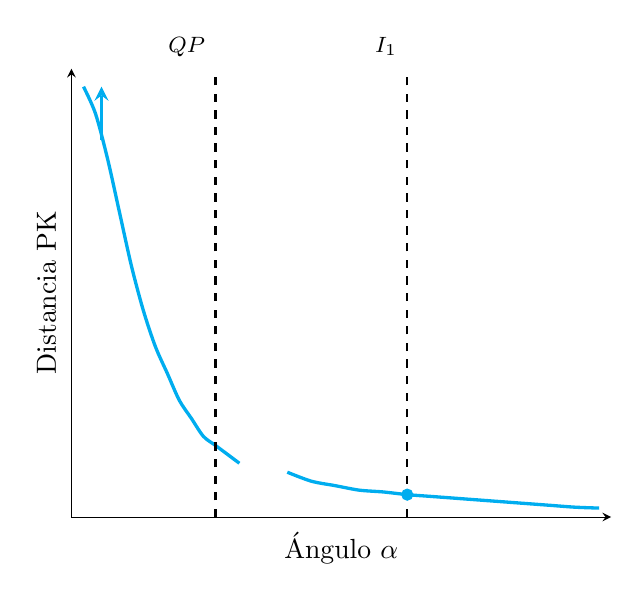
\begin{tikzpicture}[scale=1.0]
\begin{axis}[
    xlabel={Ángulo $\alpha$},
    ylabel={Distancia PK},
    xmin=0, xmax=4.5,
    ymin=0, ymax=5,
    axis lines=left,
    xtick=\empty,
    ytick=\empty,
    clip=false
]

% PRIMERA PARTE: Curva que baja dramáticamente (observación real de la imagen)
% Coordenadas extraídas visualmente de la imagen original
\addplot[cyan, very thick, smooth] coordinates {
    (0.1,4.8) (0.2,4.5) (0.3,4.0) (0.4,3.4) (0.5,2.8) 
    (0.6,2.3) (0.7,1.9) (0.8,1.6) (0.9,1.3) (1.0,1.1) 
    (1.1,0.9) (1.2,0.8) (1.3,0.7) (1.4,0.6)
};

% SEGUNDA PARTE: Después de la discontinuidad, curva MUCHO MÁS ABAJO
% Observación: La curva continúa cerca del eje X
\addplot[cyan, very thick, smooth] coordinates {
    (1.8,0.5) (2.0,0.4) (2.2,0.35) (2.4,0.3) (2.6,0.28) 
    (2.8,0.25) (3.0,0.23) (3.2,0.21) (3.4,0.19) (3.6,0.17) 
    (3.8,0.15) (4.0,0.13) (4.2,0.11) (4.4,0.1)
};

% FLECHA VERTICAL CYAN (elemento distintivo observado)
\draw[cyan, very thick, -stealth] (axis cs:0.25,4.2) -- (axis cs:0.25,4.8);

% Líneas punteadas verticales (posiciones observadas en la imagen)
\draw[dashed, black, thick] (axis cs:1.2,0) -- (axis cs:1.2,5) 
    node[left, black, yshift=8pt] {\footnotesize $QP$};
\draw[dashed, black, thick] (axis cs:2.8,0) -- (axis cs:2.8,5) 
    node[left, black, yshift=8pt] {\footnotesize $I_1$};

% Punto destacado (observado en la imagen original)
\addplot[cyan, mark=*, mark size=2pt, only marks] coordinates {(2.8,0.25)};

\end{axis}
\end{tikzpicture}

\end{document}
